\documentclass{beamer}

\usepackage[utf8]{inputenc} % ~ Encodage
\usepackage[T1]{fontenc}    % ~ Encodage
\usepackage{xcolor}   % ~ Couleurs fs
\usepackage{xmpmulti}
\usepackage{multicol}
\usepackage[many]{tcolorbox}
\usepackage[british]{babel}
\usepackage{listings}
\usepackage{array}
\usepackage{tikz}

\definecolor{darkWhite}{rgb}{0.94,0.94,0.94}


\newtcolorbox{cadre}
{
    colframe=blue!50!black,
    colback=blue!75!black,
    halign=center,
    valign=center
}

\beamertemplatenavigationsymbolsempty
\usetheme{Dresden}
\setbeamertemplate{page number in head/foot}[framenumber]

\title{Programming Scalable Systems  Project \\ BetUnfair (Betting exchange platform)}
\author{Alexandre Arabian \and Nathan Maillet}
\institute[ETSIINF]
{
    Escuela Técnica Superior de Ingenieros Informáticos\\
    Universidad Politécnica de Madrid
}
\date{}

\begin{document}

\begin{frame}
    \titlepage
\end{frame}

\section*{Implementation}
\begin{frame}{}
    \centering
    \begin{cadre}
        \textcolor{white}{
            Implementation
        }
    \end{cadre}
\end{frame}

\begin{frame}{Functional view}
    \centering
    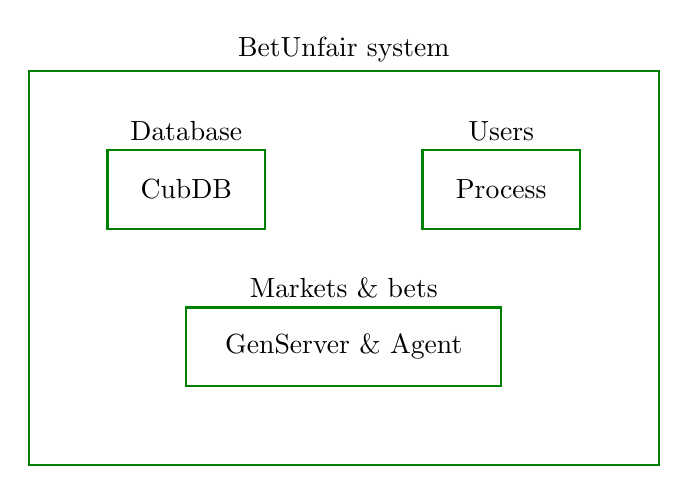
\begin{tikzpicture}
        \node[above] at (4,5) {BetUnfair system};
        \draw[thick, color=green!50!black] (0,0) rectangle (8,5);

        \node[above] at (4,2) {Markets \& bets};
        \draw[thick, color=green!50!black] (2,1) rectangle (6,2) node[midway, black] {GenServer \& Agent};

        \node[above] at (2,4) {Database};
        \draw[thick, color=green!50!black] (1,3) rectangle (3,4) node[midway, black] {CubDB};

        \node[above] at (6,4) {Users};
        \draw[thick, color=green!50!black] (5,3) rectangle (7,4) node[midway, black] {Process};
    \end{tikzpicture}
\end{frame}

\begin{frame}{Processes \& data types}
    \centering
    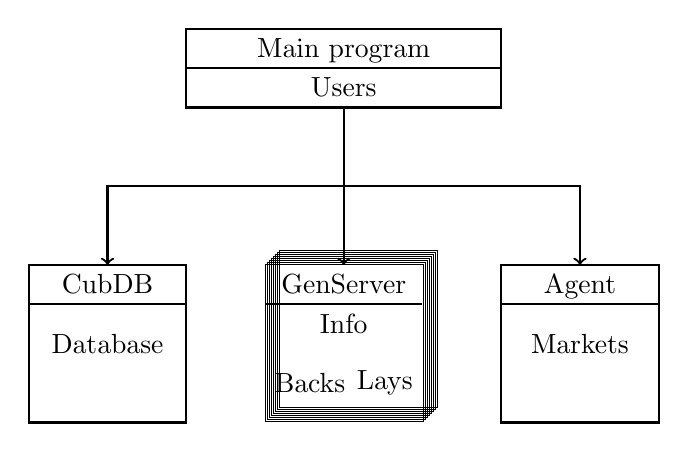
\begin{tikzpicture}
        %% Rectangles
        \draw[thick] (-2,0) rectangle (2,1);
        \draw[thick] (-4,-4) rectangle (-2,-2);
        \foreach \t in {0.01,0.035,...,0.2} {
                        \draw (-1+\t,-4+\t) rectangle (1+\t,-2+\t);
                        }
        %\draw[thick] (-1,-4) rectangle (1,-2);
        \draw[thick] (2,-4) rectangle (4,-2);

        % Arrows
        \draw[thick, ->] (0,0) -- (0,-1) -- (-3,-1) -- (-3,-2);
        \draw[thick, ->] (0,0) -- (0,-2);
        \draw[thick, ->] (0,0) -- (0,-1) -- (3,-1) -- (3,-2);

        % Titles
        \node[below] at (0,1) {Main program};
        \node[below] at (-3,-2) {CubDB};
        \node[below] at (0,-2) {GenServer};
        \node[below] at (3,-2) {Agent};

        % Separators
        \draw[thick] (-4,-2.5) -- (-2,-2.5);
        \draw[thick] (-1,-2.5) -- (1,-2.5);
        \draw[thick] (4,-2.5) -- (2,-2.5);
        \draw[thick] (-2,0.5) -- (2,0.5);

        % Data types
        \node at (-3,-3) {Database};
        \node[right] at (-1,-3.5) {Backs}; % [bet()]
        \node[above] at (0,-3) {Info}; % market()
        \node[left] at (1,-3.5) {Lays}; % [bet()]
        \node at (3,-3) {Markets}; % Map :: market_id() -> market_pid()
        \node[below] at (0,0.5) {Users};
    \end{tikzpicture}
\end{frame}


\section*{Test \& Benchmarking}
\begin{frame}{}
    \centering
    \begin{cadre}
        \textcolor{white}{
            Test \& Benchmarking 
        }
    \end{cadre}
\end{frame}

\begin{frame}{Logical tests}
    \centering
    \textbf{Functionalities of the API}\\
    \begin{tabular}{|l|l|}
        \hline Functionality & Done/Todo \\
        \hline Stop \& Restart & \(\checkmark\) \\
        \hline Management of users account & \(\checkmark\) \\
        \hline Create multiple bets for a user & \(\checkmark\) \\
        \hline Matching and settling markets & \(\checkmark\) \\
        \hline Our code passes all unit tests & \(\checkmark\) \\
        \hline
    \end{tabular}
\end{frame}

\begin{frame}{Test of scalability}
    %% TODO : graph/smthing linked to the benchmarking %%
    % 100000 -> 18
    % 10000 ->  0.7
    % 1000 ->   0.3
    \centering
    \textbf{Scalability test}\\
    \begin{tabular}{|l|l|}
        \hline Number of users & time to run \\
        \hline 1000            & 0.3 sec\\
        \hline 10000           & 0.7 sec\\
        \hline 100000          & 18  sec\\
        \hline
    \end{tabular}\\
    Parameter~: 50 users per markets
    \begin{alertblock}{Analyse}
        As we have~: \(\frac{18}{0.7} = 25.7\) and \(\frac{0.7}{0.3} = 2.3\),
        our system runs in \(\mathcal{O}(n^2)\) with \(n\) the number of users.
    \end{alertblock}
\end{frame}

\section*{Conclusion}
\begin{frame}{}
    \centering
    \begin{cadre}
        \textcolor{white}{
            Conclusion 
        }
    \end{cadre}
\end{frame}

\begin{frame}{Challenged faced}
    \begin{itemize}
        \item One of us had issues to run mix along with code from github 
        \item Difficulties in data manipulation (use of Process, Registry, Agent\dots)
        \item Problems with the tester~: namming conventions and logic of the betting place
    \end{itemize}
\end{frame}

\begin{frame}{Future ideas}
    For a future version of our application, we could add~:
    \begin{itemize}
        \item An history of bets
        \item Video streams to description of markets (live update about event)
        \item Select who can bet against you
        \item Making bets with multiple persons, dividing the cost and gains
    \end{itemize}
\end{frame}

\end{document}

% The contents of the slides should detail the design, 
% implementation, and testing and benchmarking of the project, 
% including any challenges faced and future improvements related with scalability aims.


% Challenges faced:

% We started the implementation using Processes, but found issues regarding the bets functionalities, correctly setting the ids each time for a backing and laying bet, specifically to the way we implemented it. Thus, we moved towards the use of Registry. However, we encountered errors and exceptions at runtime, which depended on the order of concurrent factors. Sometimes we would try to use a non-existent PID, other times it wouldn't recognize the Registry used, maybe we would get both errors, or none.
% Due to this, we moved to the use of Agent, which fixed the issues above.
% We encountered some problems regarding the tester. We had different understandings for how the matching of bets should really work, so we juggled between doing each tester by hand and changing our code, then changing the tester, and then back to changing the code. At the end, we cleared our doubts when we got in contact with the professor.
